% Native vector schematic of the Mask R-CNN pipeline used in this thesis.
\begingroup
% Shared visual language for the three segmentation-method diagrams.
\tikzset{
    box/.style={draw, rounded corners=2pt, align=center, font=\small,
        text width=44mm, minimum height=9mm, inner sep=4pt, line width=0.5pt},
    process/.style={box, fill=gray!7},
    model/.style={box, very thick, fill=blue!5},
    output/.style={box, dashed},
    supervision/.style={box, densely dashed, fill=gray!7},
    link/.style={->, semithick},
    traininglink/.style={link, densely dashed}
}

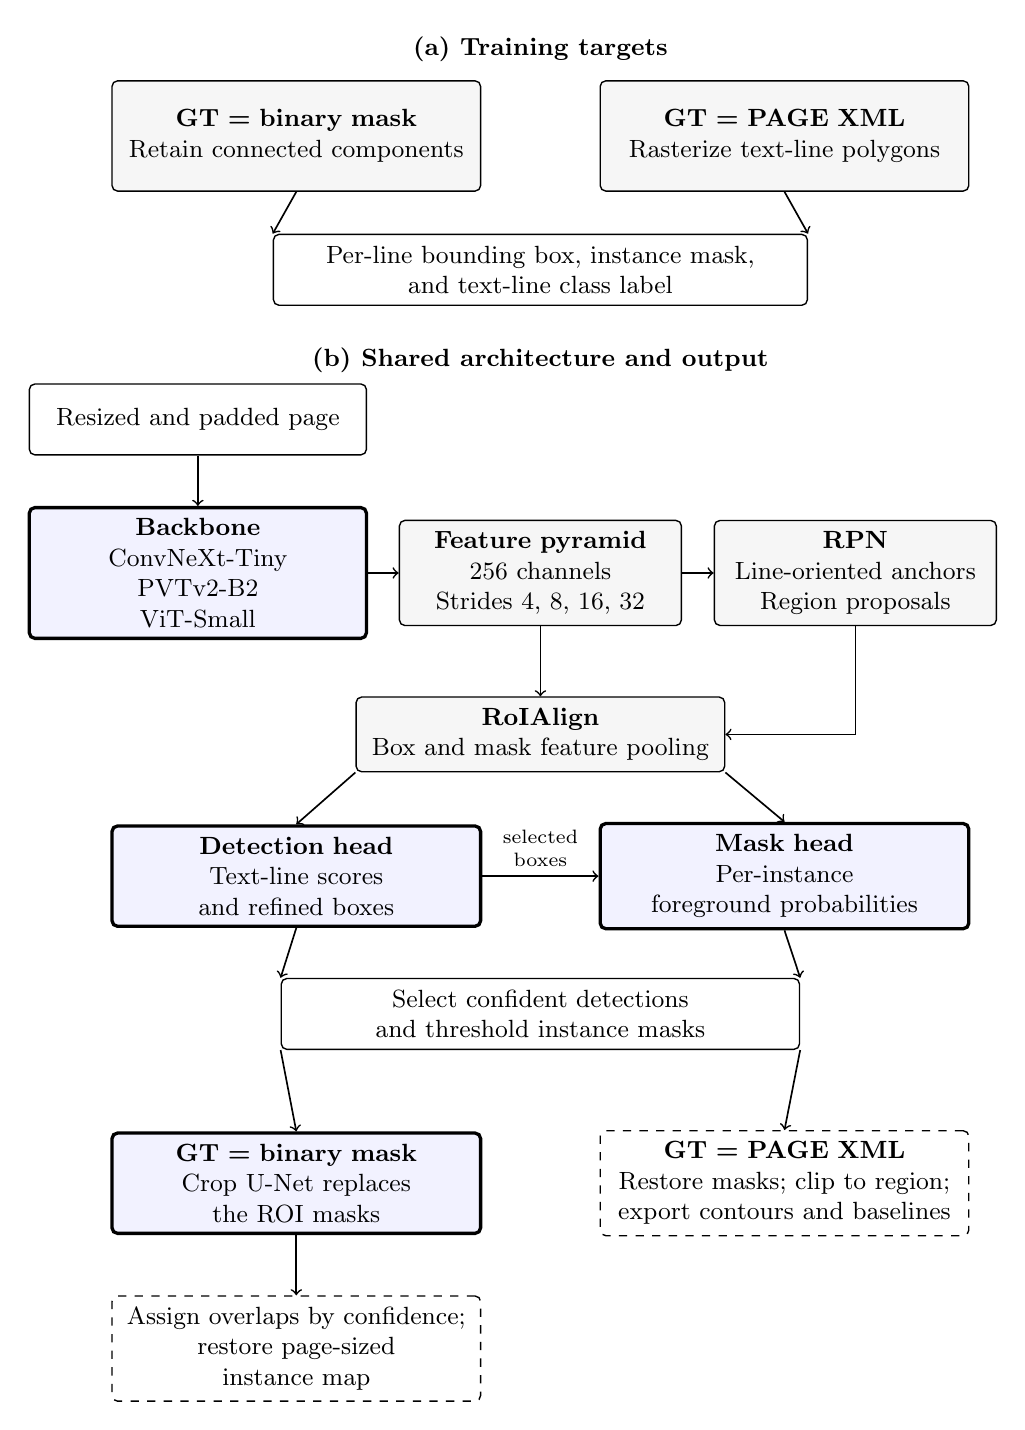
\begin{tikzpicture}
    \node[font=\small\bfseries] at (0,0.4) {(a) Training targets};
    \node[process, minimum height=14mm] (binary-gt) at (-3.1,-0.7)
        {\textbf{GT = binary mask}\\Retain connected components};
    \node[process, minimum height=14mm] (xml-gt) at (3.1,-0.7)
        {\textbf{GT = PAGE XML}\\Rasterize text-line polygons};
    \node[box, text width=65mm] (targets) at (0,-2.4)
        {Per-line bounding box, instance mask,\\and text-line class label};
    \draw[link] (binary-gt.south) -- (targets.north west);
    \draw[link] (xml-gt.south) -- (targets.north east);

    \node[font=\small\bfseries] at (0,-3.55) {(b) Shared architecture and output};
    \node[box, text width=40mm] (image) at (-4.35,-4.3)
        {Resized and padded page};
    \node[model, text width=40mm] (backbone) at (-4.35,-6.25)
        {\textbf{Backbone}\\ConvNeXt-Tiny\\PVTv2-B2\\ViT-Small};
    \node[process, text width=33mm] (fpn) at (0,-6.25)
        {\textbf{Feature pyramid}\\256 channels\\Strides 4, 8, 16, 32};
    \node[process, text width=33mm] (rpn) at (4.0,-6.25)
        {\textbf{RPN}\\Line-oriented anchors\\Region proposals};
    \node[process, text width=44mm] (roi) at (0,-8.3)
        {\textbf{RoIAlign}\\Box and mask feature pooling};
    \node[model] (box-head) at (-3.1,-10.1)
        {\textbf{Detection head}\\Text-line scores\\and refined boxes};
    \node[model] (mask-head) at (3.1,-10.1)
        {\textbf{Mask head}\\Per-instance\\foreground probabilities};
    \node[box, text width=63mm] (predictions) at (0,-11.85)
        {Select confident detections\\and threshold instance masks};
    \node[model] (crop-refine) at (-3.1,-14.0)
        {\textbf{GT = binary mask}\\Crop U-Net replaces\\the ROI masks};
    \node[output] (binary-out) at (-3.1,-16.1)
        {Assign overlaps by confidence;\\restore page-sized instance map};
    \node[output] (xml-out) at (3.1,-14.0)
        {\textbf{GT = PAGE XML}\\Restore masks; clip to region;\\export contours and baselines};
    \draw[link] (image) -- (backbone);
    \draw[link] (backbone) -- (fpn);
    \draw[link] (fpn) -- (rpn);
    \draw[link] (fpn) -- (roi);
    \draw[link] (rpn.south) |- (roi.east);
    \draw[link] (roi.south west) -- (box-head.north);
    \draw[link] (roi.south east) -- (mask-head.north);
    \draw[link] (box-head.east) -- node[above, font=\scriptsize, align=center]
        {selected\\boxes} (mask-head.west);
    \draw[link] (box-head.south) -- (predictions.north west);
    \draw[link] (mask-head.south) -- (predictions.north east);
    \draw[link] (predictions.south west) -- (crop-refine.north);
    \draw[link] (crop-refine) -- (binary-out);
    \draw[link] (predictions.south east) -- (xml-out.north);
\end{tikzpicture}
\endgroup
